\def \methodname {TeAR\xspace}
\def \methodnamefull {Telemetry Assisted Racing\xspace}

\chapter{Design and Implementation}
This chapter provides a detailed description of the design and implementation of the software artefact employed in this project. The chapter starts by giving an overview of the core requirements for the main software artefact which we refer to as \emph{\methodnamefull (\methodname)} (see Section \S\ref{sec:imp-requirements}). Section \S\ref{sec:imp-supportingTools} discusses the tools developed to create content for the feedback system, including track annotation and racing line visualisation amongst others \S\ref{sec:imp-supportingTools}. The chapter concludes with an in-depth description of the internals of the feedback system, the respective components, their integration and communication \ref{sec:imp-systemArchitecture}.

\section{Requirements}
\label{sec:imp-requirements}
Deliberation on the methodologies provided in Chapter \ref{chp:methodology} led to a number of requirements being identified for the software artefact. These requirements are listed below:

\begin{itemize}
	\item Content creation and annotation 
	\item Interfacing with third-party racing sim software 
	\item Efficiently read and process incoming telemetry stream
	\begin{itemize}
		\item Filter the stream for noise and unnecessary detail
		\item Structure raw data to facilitate further processing
	\end{itemize}
	\item Develop a heuristic-based system to provide feedback
	\item Provide a mechanism for communicating feedback to user
	\item Persist telemetry data for further processing
\end{itemize}

Circuit information coming from third-party software, such as the racing line, must be available to \methodname; furthermore, this data is to be annotated with additional information such as track section partitioning and the respective properties, which are fundamental in determining which feedback to provide to the user. Thus, a number of supporting tools have to be developed.
\methodname must interface with the third party racing simulation software (Assetto Corsa) via the inter-process communication system provided by the program. In addition, \methodname must extract a stream of telemetry data from the simulator, at a sampling rate of approximately 333Hz (which is the sustained rate provided by Assetto Corsa).
The incoming telemetry data must be filtered since not all data is useful to \methodname. Furthermore, these data are organised into structures that are more conducive to processing later on in the pipeline. 
This telemetry information will be fed into a heuristic-based algorithm that should return feedback that will eventually be presented to the user. This feedback should be the most effective correction the user would need to make to improve that particular race track section.
\methodname should communicate this feedback to the user via an auditory messaging system. 
Finally, all telemetry data should be persisted onto secondary storage for offline analysis. 

%The following core requirements have been identified for \methodname:
%\begin{description}
%	\item[Abstract Input/Output Interface] The telemetry data input and feedback output needs to be abstracted. Techniclay this does not effect the feedback's effectiveness or accuracy but it is usefull as to be able to change the sim racing game and the type of feedback which is given with out having to change any of the internal components. This allows for fast prototyping especially with the output interface in which one can develop another way to convey the feedback. 
%	\item[Perform Spatial Querying] The feedback system relies on being able to determine the location of the car on track. This is used to determine if the car is in a straight section or corner section, how far away from the race line the car is and if the mid point of the corner is being driven on. 
%	\item[Store telemetry files] In order for the evaluation chapter to be carried out, the telemetry data is required to be stored for later data analysis. This is achieved by writing the telemetry data to a log file which is later uploaded to the database.
%	\item[Query log files]
%\end{description}

\section{Content Creation and Annotation}
\label{sec:content-creation}
The telemetry data stream read-out from Assetto Corsa does not provide sufficient information about the environment for \methodname to make informed decisions about possible feedback. The feedback mechanism used in \methodname is highly dependent on the racing line, which in turn, is a function of the track geometry; however, it is not possible to acquire any meaningful information about the racing track from telemetry data alone. These factors prompted the creation of the \emph{Track Splicer and Visualiser}, a supporting tool that extracts track information from the Assetto Corsa data files and provides additional annotations to this data as required by \methodname. 

\subsection{Track Splicing}
\label{sec:imp-trackSplicer}
The track splicing tool extracts track and racing line information from Assetto Corsa, partitions the data into a number of sections that are annotated as either straight or corner, and finally finds the apex of each corner section. The tool also provides visualisation of the results in case the user needs to tweak the generation parameters. This process is shown in Figure \ref{fig:diagram-trackspliceinputoutput}.

%The track splicer tool has been developed to aid the feedback system's track meta data file creation. It automates the following tasks. Given a series of two dimensional cartesian coordinate denoting a track race line, (i) split the race line into straights and corners (ii) find the mid point of a corner which is used as the apex point and (iii) give a visual representation of the race line, straights and corners. 

\begin{figure}[!htb]
	\centering
	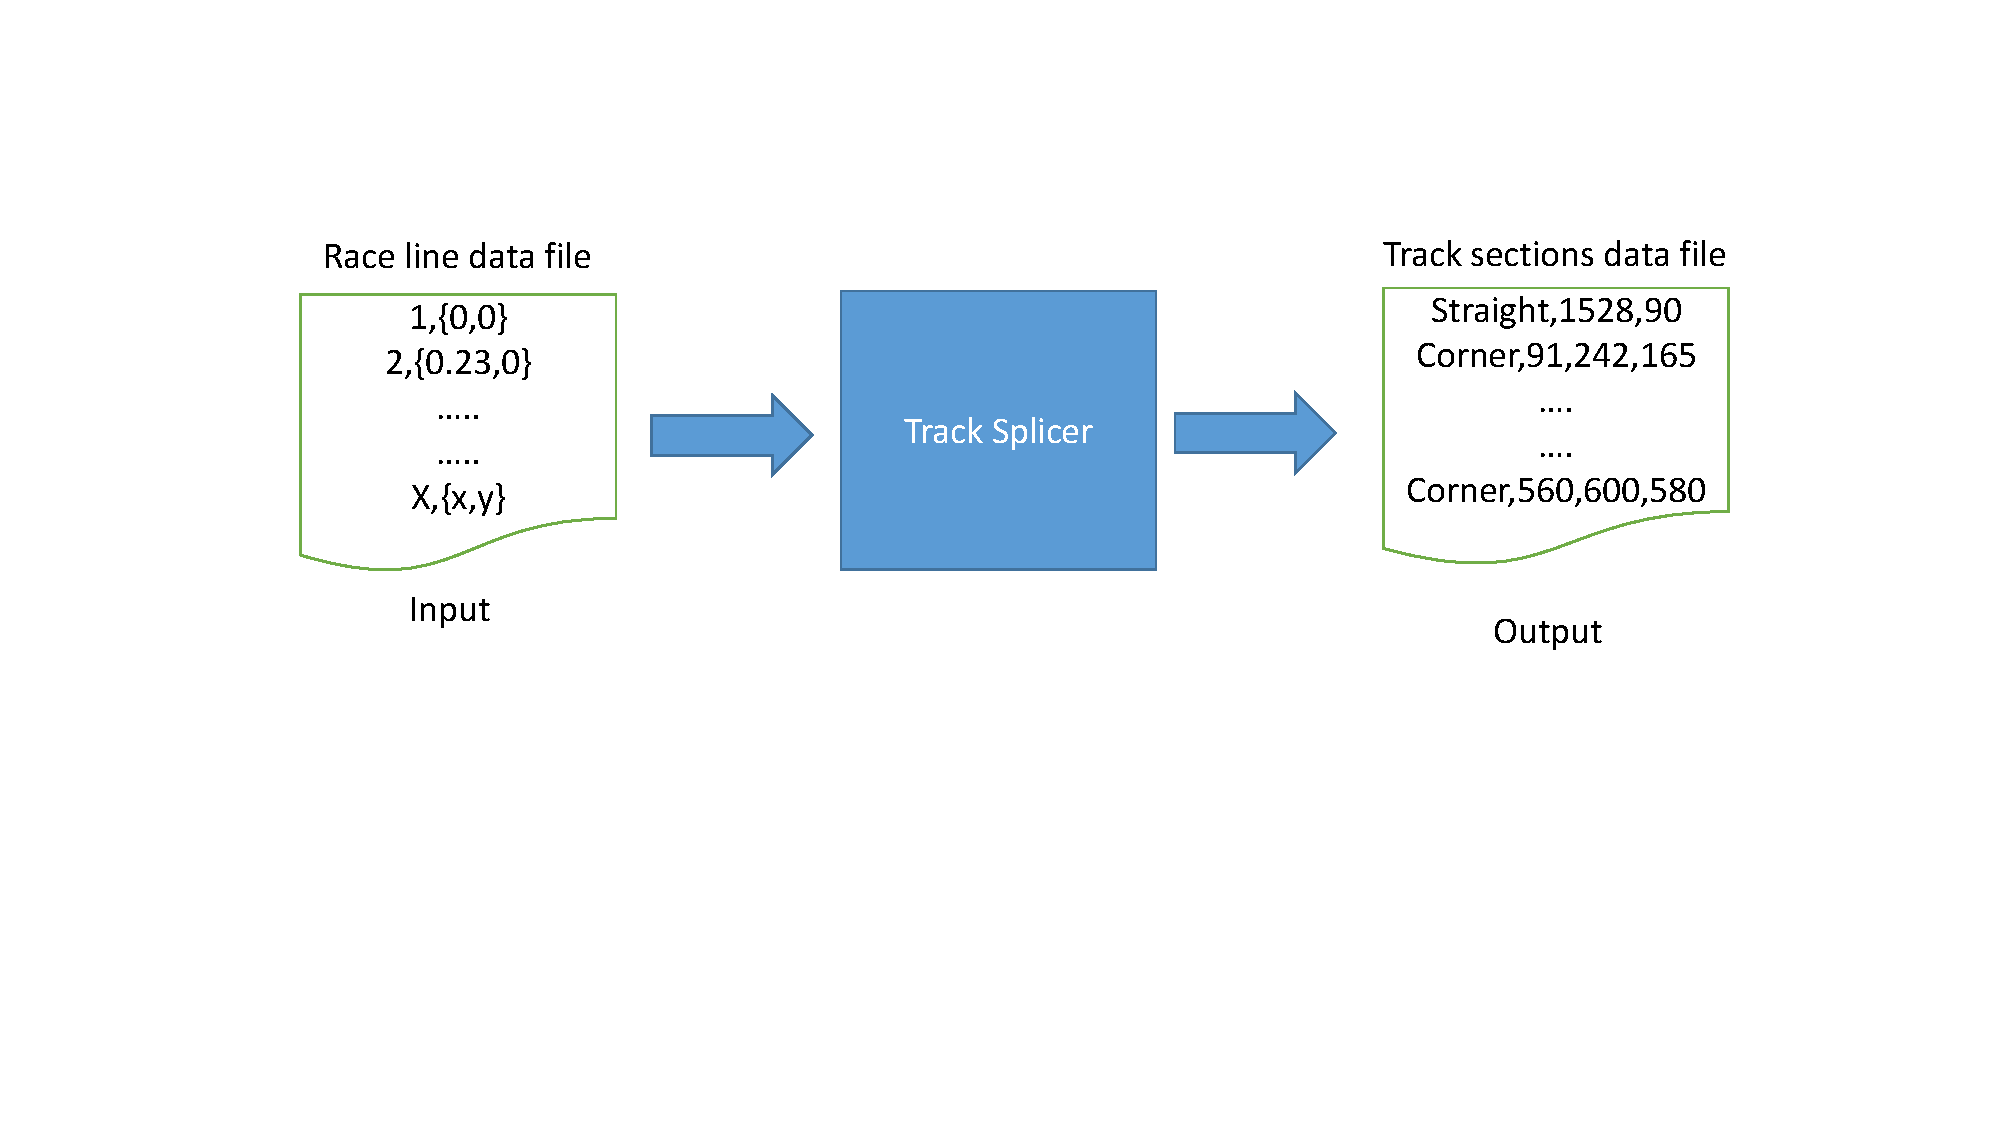
\includegraphics[width=\textwidth]{diagrams/trackspliceinputoutput.pdf}
	\caption[track splicer input out]{Track splicer input and output}
	\label{fig:diagram-trackspliceinputoutput}
\end{figure}

\begin{description}
	\item [Track Partitioning and Annotation] The idealised racing line is a simple closed curve $\mathcal{C}$ on a plane; its digital counterpart is a discrete simple closed curve $\mathcal{C}_d$ with a finite number of vertices, each lying on the curve $\mathcal{C}$ and connected by straight edges - an inscribed polygon - where each vertex $\mathbf{v}_i \in \mathcal{C}_d$ represents a coordinate pair $(x,z)$. The ground is assumed to be a horizontal plane. 	To determine whether a section of the track near a vertex $\mathbf{v}_j \in \mathcal{C}_d$ is a straight or a corner, two further vertices are sampled $\mathbf{v}_i, \mathbf{v}_k \in \mathcal{C}_d$, where $i < j < k \in \mathbb{Z}/|\mathcal{C}_d|\mathbb{Z}$. We define the measure of curvature $c_j$ for the curve at $\mathbf{v}_j$ as follows:
	\begin{equation}
		c_j = \cos^{-1} \left(\frac{\mathbf{v}_k - \mathbf{v}_j}{|\mathbf{v}_k - \mathbf{v}_j|} \cdot \frac{\mathbf{v}_j - \mathbf{v}_i}{|\mathbf{v}_j - \mathbf{v}_i|} \right),
	\end{equation}
	where $c_j$ is the angle between the two normalised unit vectors formed by the ordered vertices $\mathbf{v}_i$ through $\mathbf{v}_k$. A threshold value $c_t$ determines whether the curve segment from $\mathbf{v}_i$ through $\mathbf{v}_k$ is a corner or a straight. A typical value for $c_t$ is 0.01. Edges between consecutive vertices in $\mathbf{C}_d$ may vary in length; therefore, when vertices $\mathbf{v}_i$ and $\mathbf{v}_j$ are chosen, Poisson-Disc sampling is employed, to guarantee that the vertices are no closer to each other than a specified minimum distance $c_m$ (a typical value for $c_m$ is 5).  	

%	\item [Split the race line into straights and corners] This is done by calculating the rate of change of the line by means of vectors dot products. A cartesian coordinate p[x] as 'p1' is considered where x is the position in the array. Two other points are required p[x+1] as 'p2' and p[x+2] as 'p3'. When x is the end of the list, the first two points are used from the list. Using p1, p2 and p3, two vectors are generated, 'v1' which is a vector going from p1 to p2, and 'v2' which is a vector going from p2 to p3. The vectors are normalised as the their magnitude is irrelevant for this computation. The dot product of v1 and v2 is computed, the result is passed through the arccos function which results in the angle difference. If the angle is above a threshold value the point p1 is said to be part of a corner section, otherwise p1 is said to be part of a straight. The threshold value is customizable and is find tuned on a track by track bases.
	
	\begin{figure}[!htb]
		\centering
		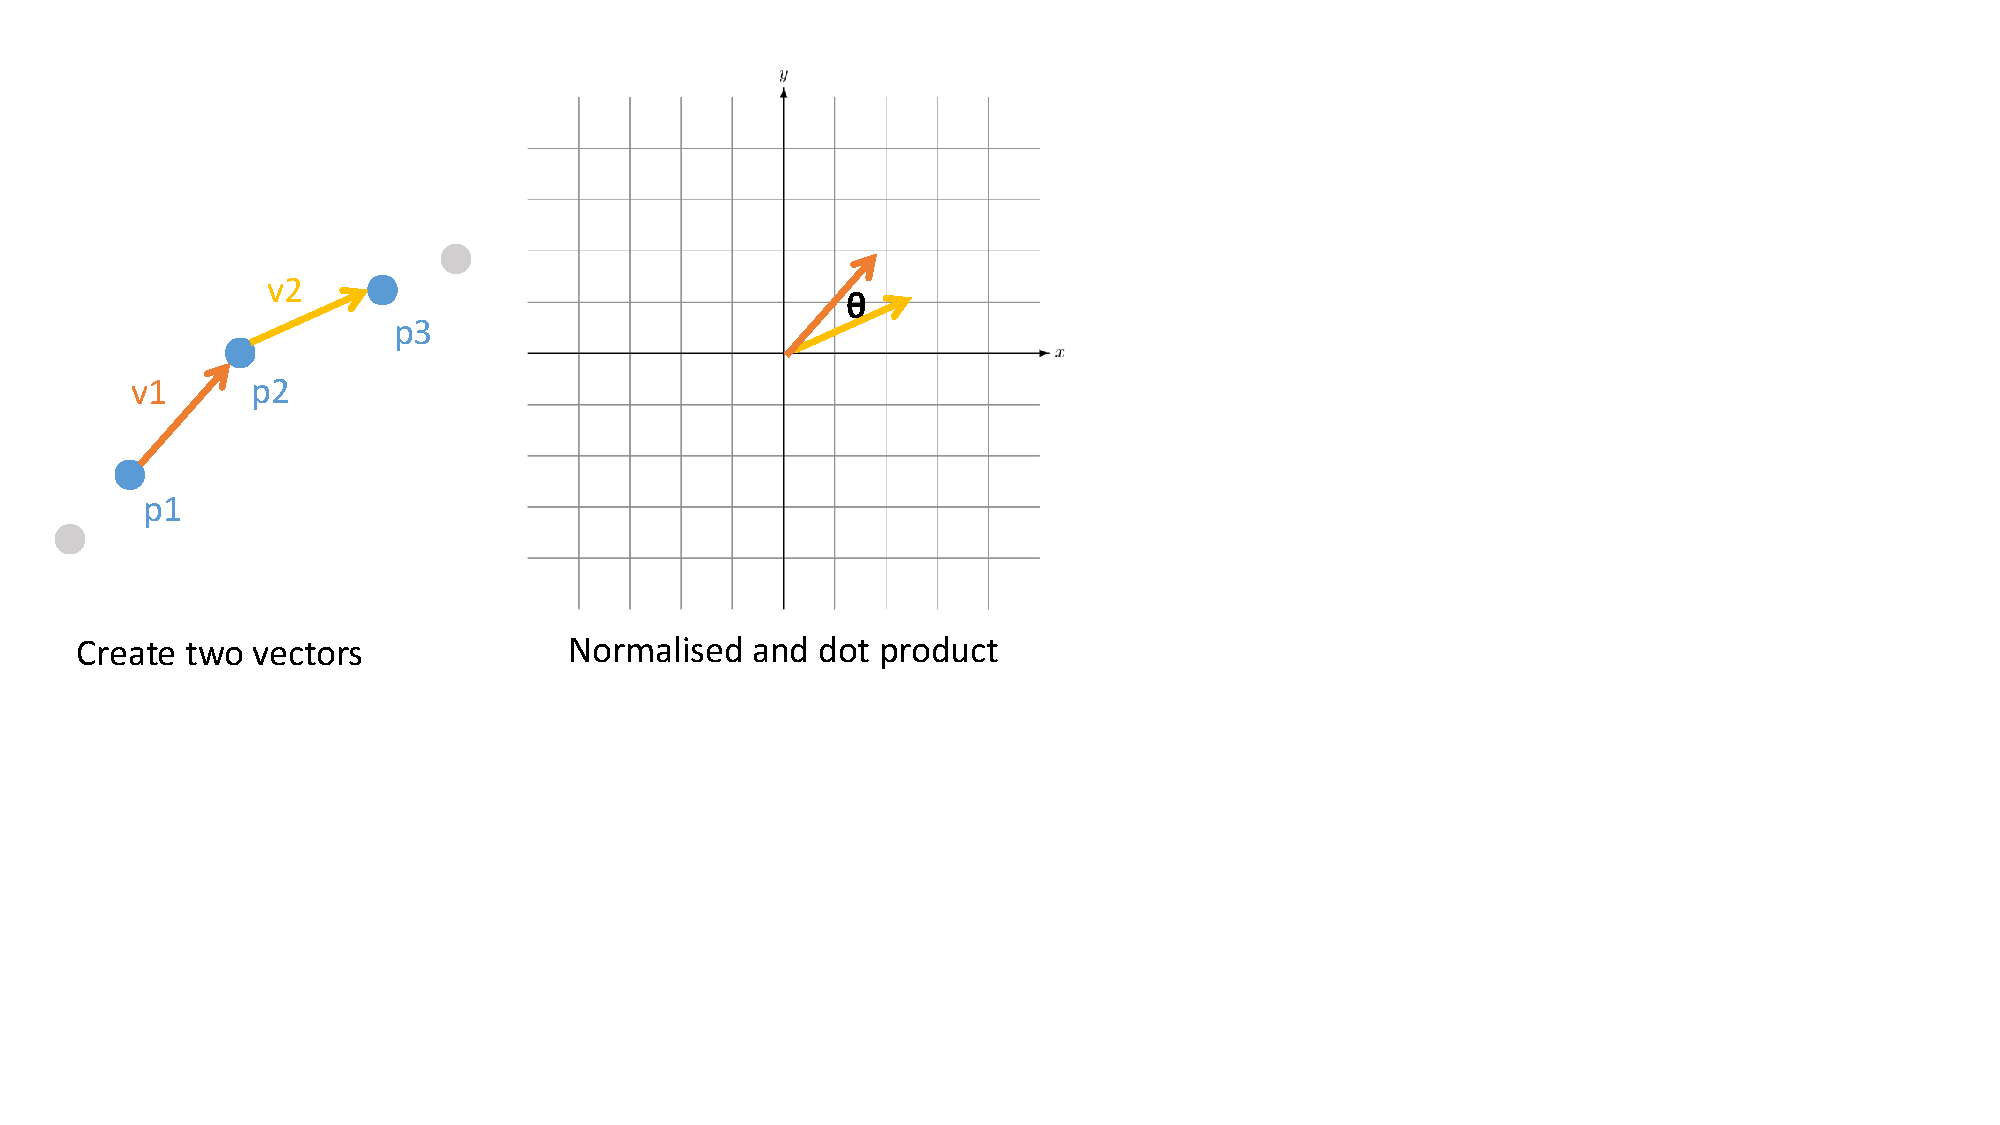
\includegraphics[width=\textwidth]{diagrams/vectorCorners.pdf}
		\caption[Splicing using vectors]{Points and vectors visualised}
		\label{fig:diagram-vectorCorners}
	\end{figure}
	
	\item [Find the mid point of a corner] The mid point of a corner is the highest point of the corner as shown in the figure. The mid point is found by going through each point. A perpendicular vector 'vP' to the first point is calculated, then a vector list vL is created containing a vector for each point as such v[x] = vector(p[x].x, p[x].y) where x is the position of the point in the array. Finally each vector in vL has the dot product with VP computed. The vector with the highest dot product result corresponds with the point which is the mid point of the corner.
	
	\begin{figure}[!htb]
		\centering
		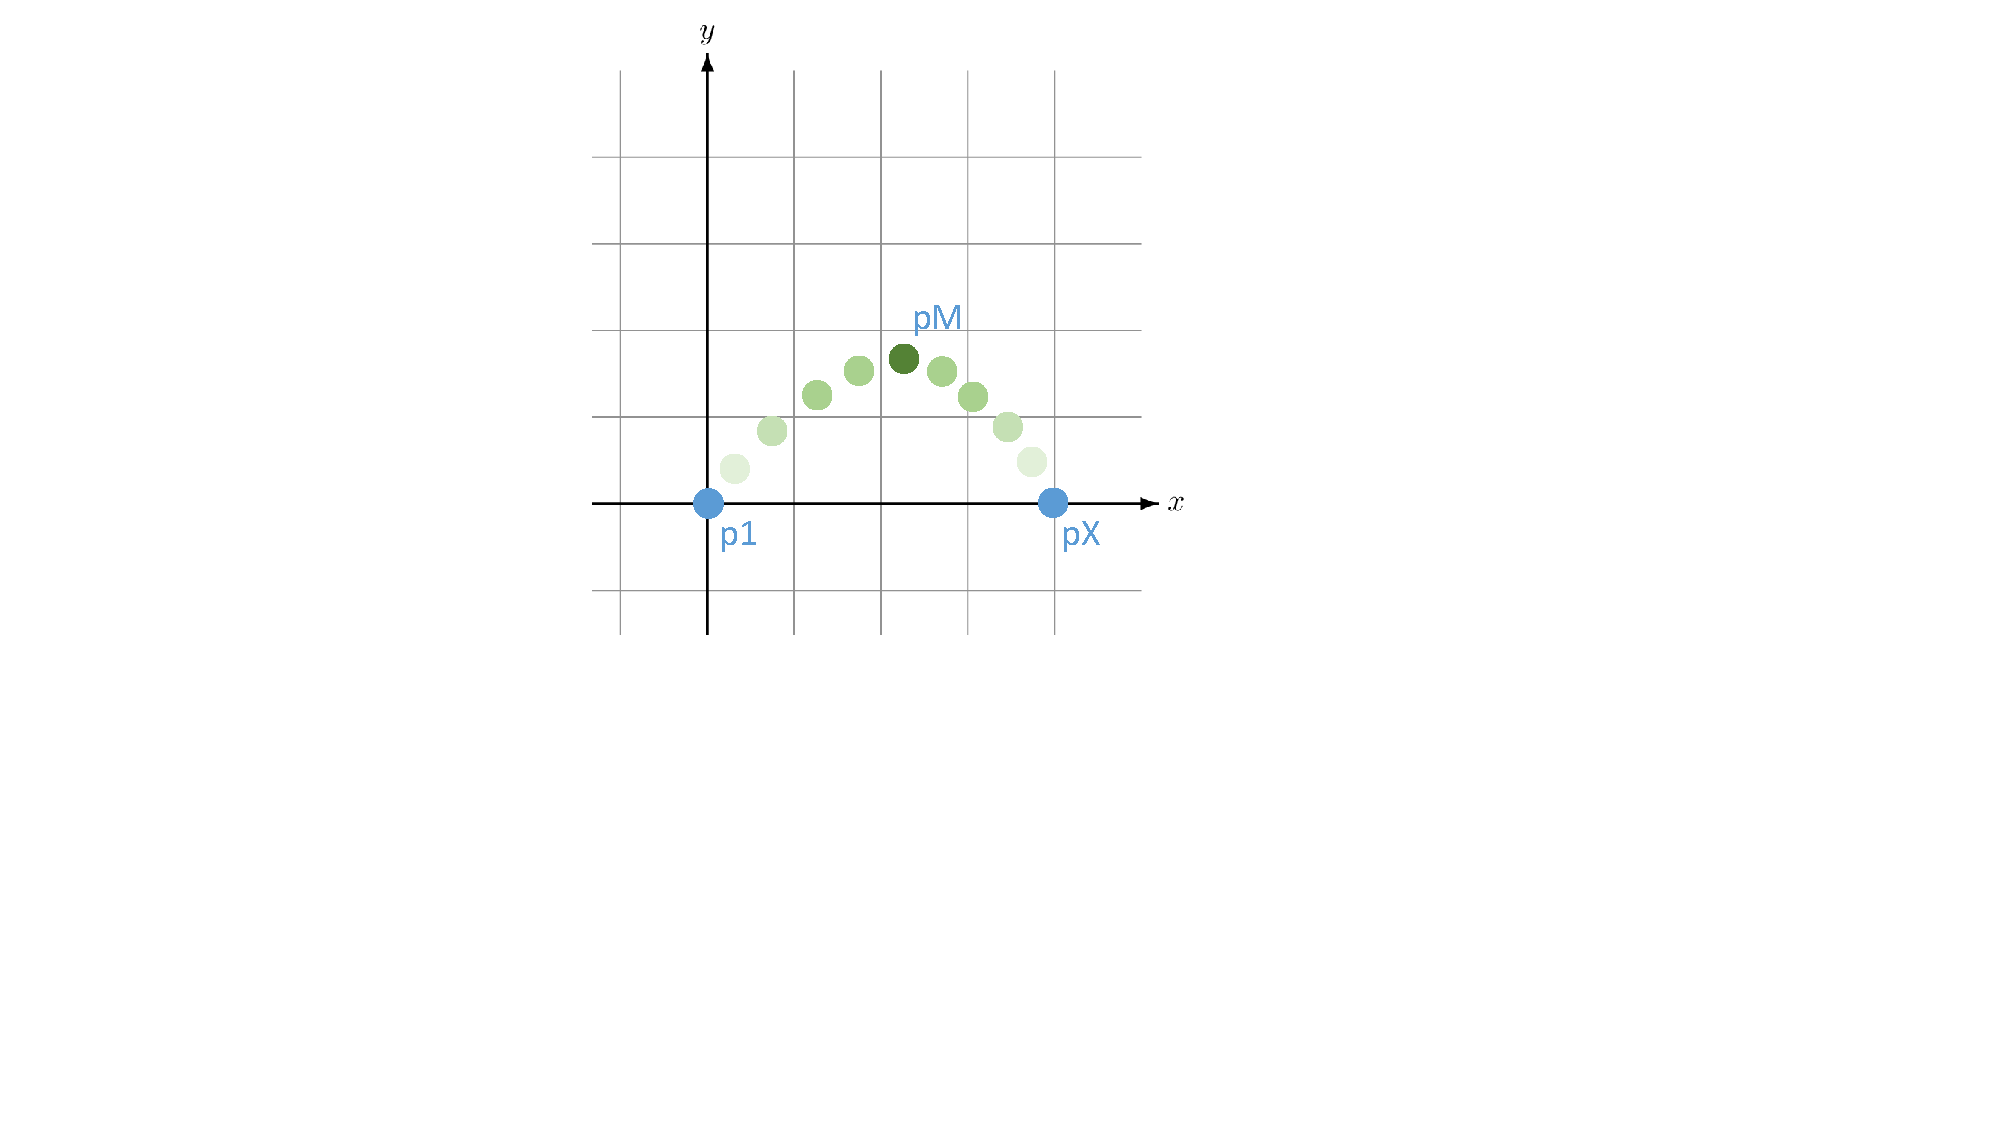
\includegraphics[height=5cm]{diagrams/cornerMidPoint.pdf}
		\caption[Corner mid point]{Finding the corner mid point}
		\textbf{p1} : First point \textbf{pM} : Corner mid point \textbf{pX} : Last point
		\label{fig:diagram-cornerMidPoint}
	\end{figure}
	
	\item [Visual representation of the race line] It was important to be able to visualise the results of the above processes in order to be able to determine the correctness of the processes. For this reasons an application with a graphic user interface was developed from which one can see the results.
	
	\begin{figure}[!htb]
		\centering
		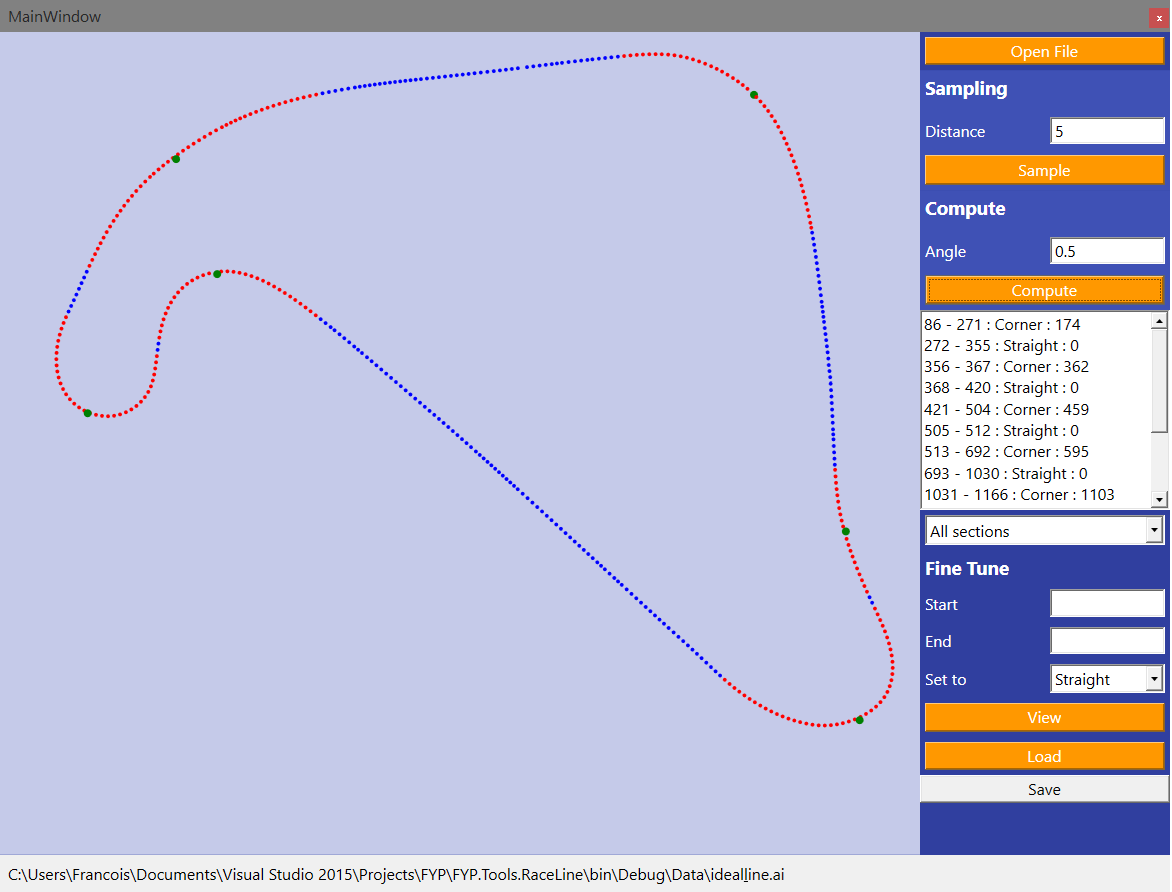
\includegraphics[height=5cm]{images/tracksplicertool}
		\caption{Track splicer tool}
		\textbf{Blue dots} : Part of a straight \textbf{Red dots} : Part of a corner \textbf{Green dots} : Corner mid point
		\label{fig:TrackSplicerTool}
	\end{figure}
	
\end{description}

\subsection{Persistence of Telemetry Data}
Log files containing telemetry data from each user session are inserted into a database management system for offline analysis. An extraction transfer loading (ETL) process (see Figure \ref{}) was purposely built, which takes as input a log file and inserts processed data as records into a database. This database is then used to run SQL queries related to the evaluation of the experiment.

\begin{figure}[!htb]
	\centering
	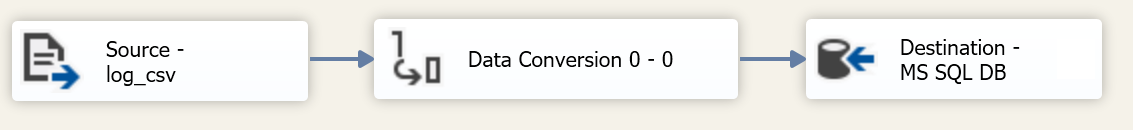
\includegraphics[width=\textwidth]{diagrams/ssis.png}
	\caption{Microsoft Integration Services SQL import}
	\label{fig:ssis}
\end{figure}

\subsection{Spatial Queries}
\label{sec:imp-SpatialQuerying}
In order for \methodname to determine the closest point on the racing line from the car's current position a spatial querying mechanism is required. Since TeAR provides real-time feedback on how the user is following the racing line, spatial queries are continuously carried out. Therefore, rather than using a linear search, a quad-tree data structure \cite{} is used to store all the points on the racing line (see Figure \ref{}) and accelerate to $\mathcal{O}(\log{n})$ spatial queries. 

\begin{figure}[!htb]
	\centering
	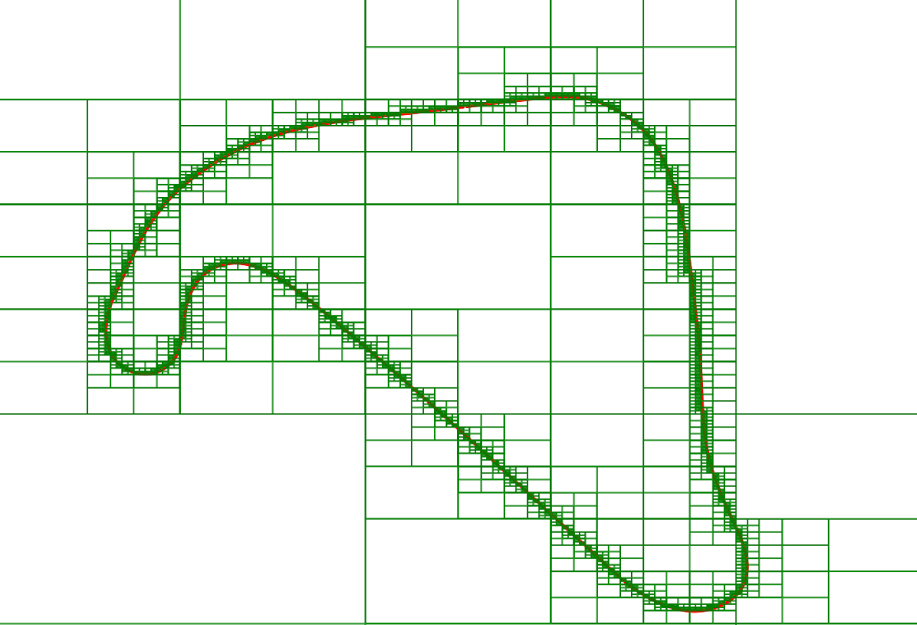
\includegraphics[height=5cm]{images/QuadTree}
	\caption{Visual representation for part of the quad tree for the Silverstone national circuit}
	\label{fig:QuadTree}
\end{figure}

\section{System Architecture}
\label{sec:imp-systemArchitecture}
The feedback system is made up of independent components which pass data to each other in order to produce the feedback instruction which is output to the user. Below is the break down of each component including an overview of their inner workings.

\begin{figure}[!htb]
	\centering
	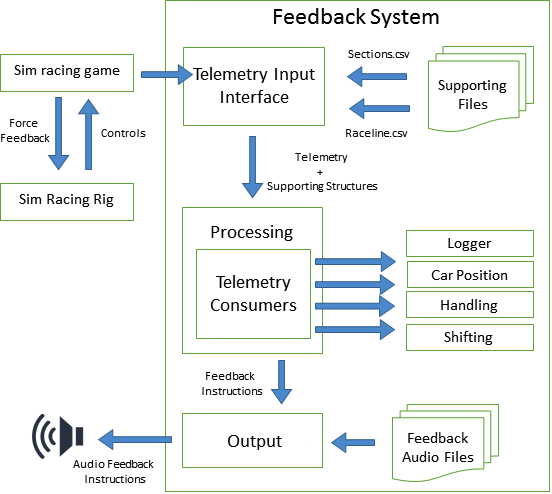
\includegraphics[height=10cm]{images/SystemArch}
	\caption{Overview of the system architecture components}
	\label{fig:SystemArch}
\end{figure}

\subsection{Telemetry Input Interface}
This components handles data inputs, two type of inputs are required, static and real time inputs. The static inputs are the ones which have been previously generated by the supporting tools. Real time input refers to the telemetry generated from the sim racing game. Assetto corsa provides a UDP server which a client can connect to, once the connection is established the game will send telemetry data.

\subsection{Processing}
Feedback processing is split into sub modules. Each module runs on a separate independent thread and gets a copy of the telemetry data passed in real time as it becomes available. Modules can be developed and plugged in without changing any other components. Having each module run on a dedicated thread ensures the system can scale horizontally making uses of all the available cores without hindering the feedback systems responsiveness. The processing component acts as a coordinator by passing data to sub modules, and listening to any feedback notification raised which are forwarded to the output interface.

\begin{figure}[!htb]
	\centering
	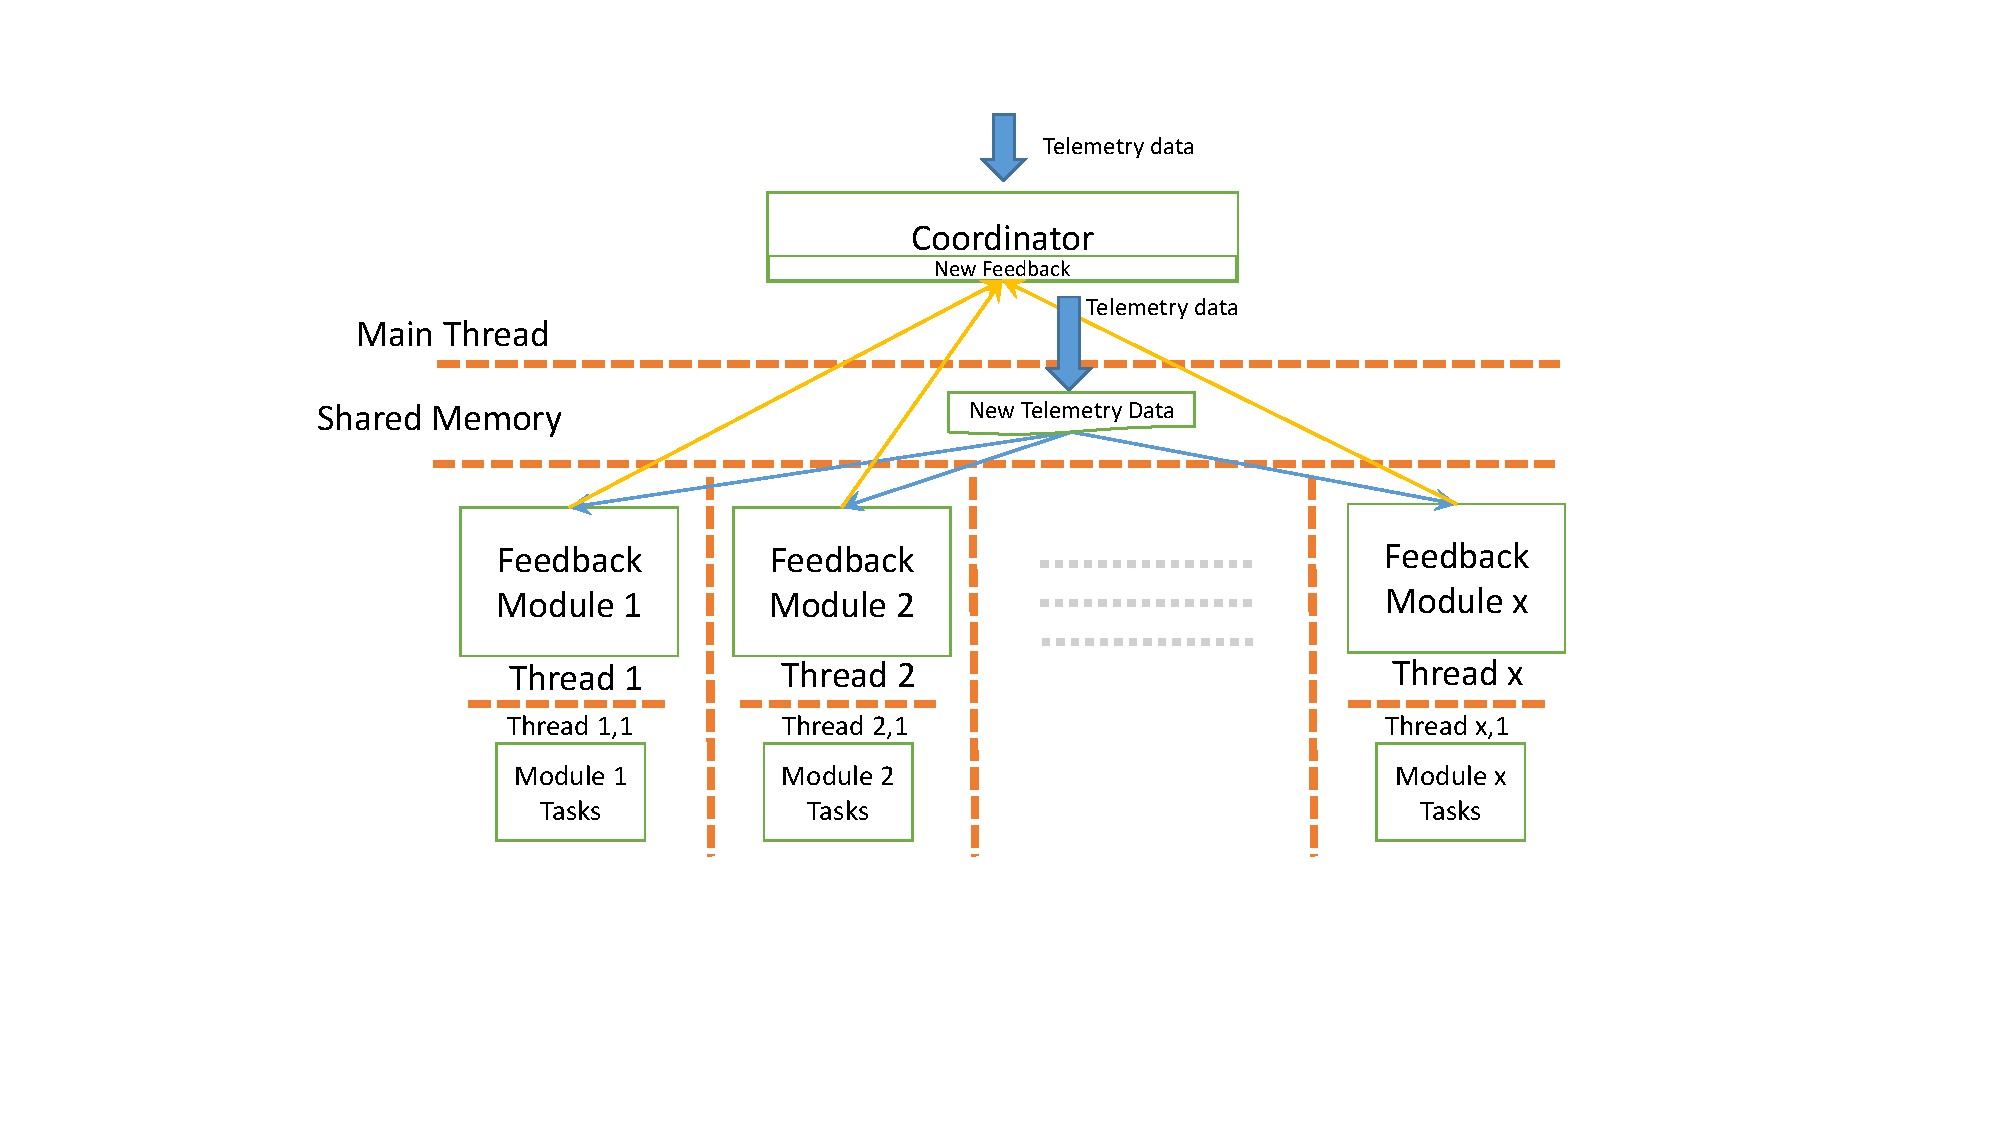
\includegraphics[width=\textwidth]{diagrams/multithreading.pdf}
	%[height=7cm]{diagrams/multithreading.pdf}
	\caption{Overview of the coordination threading}
	\label{fig:multithreading}
\end{figure}

Optimisation is also carried out within this component. This is achieved by filtering out by an expert system the feedback before being propagated to the output module. The knowledge base of the expert system is a hand crafted static one, based of rules and facts derived from the Background chapter. The inference engine works in a tiered skill based manner. At first only instructions from the basic tier are given. After the user manages to improve the basic tier skills, feedback instructions for the next tier are allowed pass to the output. In addition each module has a tolerance associated to each feedback notification it can provide. This allows the expert system to adjust how strict a module should be in raising a notification and be able to gradually make the system stricter as the user improves.

\subsection{Feedbacks being provided}
In this sub section an overview of all implemented feedback modules is given.

\textbf{Handling} component monitors for braking and acceleration behaviours. It is able to raise the following feedback notifications, 
\begin{itemize}
	\item Braking too hard
	\item Braking too light
	\item Braking in corner
	\item Losing traction to the drive wheels by applying too much power
\end{itemize}

\textbf{Car Position} component monitors for any issues which might cause the user to not adhere to the race line. As such this module can raise the following notifications 
\begin{itemize}
	\item Incorrect race line during corner
	\item Being too aggressive during a corner
	\item Not slow during a corner
	\item Track section report
\end{itemize}

\textbf{Shifting} component monitors how the user is changing gears, which allows it to raise the following notifications
\begin{itemize}
	\item Changing gear to soon
	\item Changing gear to late
	\item Taking too long to transition from one gear to another
\end{itemize}

\subsection{Output Interface}
Each possible feedback instruction which can be generated by the processing module has a static audio file associated to it. The audio files are generated from a free on line text to speech tool. The purpose of this component is to listen for feedback instruction generated by the processing component and play the corresponding audio file.